\chapter{Grundlagen} \label{chapter_2}
Für ein besseres Verständnis und genauere Definition wird das Produkt zu Beginn beschrieben. Darauf aufbauend wird der Einsatz von Produktkonfiguratoren in diesem Segment behandelt. Mobile Anwendungen stellen die dritte Grundlage für diese Arbeit.

\section{Produkt}
Im Marketing wird ein Produkt als Ergebnis im Produktionsprozess definiert. Innerhalb des Prozesses entsteht  das Produkt, welches am Ende eine Summe mehrerer materieller oder immaterieller Eigenschaften besitzt \cite{bib:product}. Aus Sicht des Kunden ist ein solches Produkt ein Einzelstück, das für die Befriedigung eines Nutzens eingesetzt werden kann. Ein konkretes Produkt ist bspw. ein Auto, da es ein Resultat eines Produktionsprozesses ist. Ein Kunde nimmt das Produkt als einzelnes Objekt wahr. Bei der Produktion hingegen ist das Auto eine Zusammenstellung aus mehreren Einzelteilen. Hier besteht ein Auto aus den vier Hauptbereichen Karosserie, Motor, Innenausstattung und Getriebe. Die Innenausstattung besteht wiederum aus Sitzen und Armaturen. Diese Verfeinerung ist die Basis für die Individualität eines bestimmten Produktes. Je mehr Verfeinerungen existieren, umso komplexer ist das einzelne Produkt. Sobald der Hersteller mehr als eine Variante einer Einzelkomponente für den Kunden zur Verfügung stellt, lässt sich ein Produkt individualisieren. Dies wird wie eingangs schon erwähnt als mass-customization bezeichnet. \par 

Voraussetzung für diesen Trend ist eine veränderte Wahrnehmung des Kunden. Das Produkt darf nicht mehr als einzelnes Objekt gesehen werden. Für die individuellen Anpassung muss der Kunde das Produkt als eine Zusammenstellung mehrerer Komponenten verstehen. Diese veränderte Wahrnehmung gilt es dem Kunden zu vermitteln und ihm dadurch eine Individualisierung seines Produktes zu ermöglichen. \par

Die zweite große Herausforderung entsteht bei baulichen Abhängigkeiten der einzelnen Produktteile. Bei einem komplexen Produkt mit vielen Einzelteilen können viele Abhängigkeiten entstehen. Wenn bei einem Auto bspw. ein bestimmter Motor ausgewählt wurde, so lassen sich nur für den Motor passende Getriebe einbauen. Durch die Verwendung mehrerer Möglichkeiten für eine bestimmte Einzelkomponente steigt ebenfalls die Anzahl der Abhängigkeiten. Die Prüfung dieser Abhängigkeiten muss ein Experte durchführen, der sich bestens mit der Produktzusammensetzung auskennt. Damit die einzelnen Vorgänge nicht zu komplex werden, müssen geeignete Formen der Darstellung gefunden werden.

\subsection{Produktkatalog}
Um dem Kunden einen Einblick in das Produkt zu verschaffen werden sogenannte Produktkataloge verwendet. Diese Kataloge sind meist in Papierform vorhanden und enthalten für den Kunden relevante Informationen über das Produkt. 

Für die Zusammenstellung eines Produktes benötigt der Kunde ein geeignetes Hilfsmittel. Ein solches Hilfsmittel kann ein Produktkatalog sein. In einem Katalog werden die einzelnen Komponenten eines Produktes dargestellt.  


\subsection{boolesche Logik in der Produktmodellierung}


\section{Produktkonfiguratoren}\label{konfiguratoren}
Das Ziel des Produktkonfigurators ist es, produktspezifisches Wissen für die Anwender bereit zu stellen. Dieses hilft beim individuellen Zusammenstellung des Produktes. Ein solches System wird in die Kategorie der Expertensysteme\cite{bib:puppe} oder wissensbasierte Systeme eingeordnet. Der Aufbau eines solches System ist in Abbildung \ref{expert_system_structure} zu sehen. \par
\begin{figure}
\centering
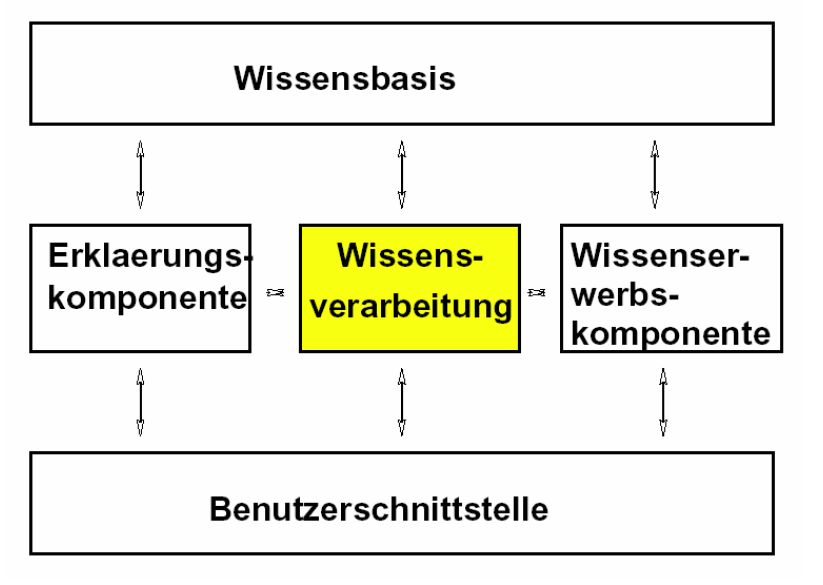
\includegraphics[width=250px]{images/expertensysteme}
\caption{Aufbau eines Expertensystems \cite[s.6]{bib:keller}}
\label{expert_system_structure}
\end{figure}

Die zentrale Komponente ist die \textit{Wissensverarbeitung}. Diese hat auf alle weiteren Komponenten Zugriff und interagiert mit diesen. Es werden die erhaltenen Fakten mithilfe der vorhandenen Regeln verknüpft. Aus der Verknüpfung werden neue Fakten gewonnen, die auf der \textit{Benutzerschnittstelle} angezeigt werden. Die Wissensbasis ist für das Speichern des Expertenwissens in Fakten und Regeln zuständig. Die Speicherung der Daten kann auf folgende zwei Arten geschehen\cite{bib:expert1}:\par
\begin{itemize}
        \item \textbf{generisch}: unabhängig vom aktuellen Anwendungsfall. Meist in einfachen Wenn-Dann-Regeln oder auf einem Modell beruhend. 
        \item \textbf{fallspezifisch}: zur Lösung eines konkreten Anwendungsfall
\end{itemize}
 Die Pflege dieser Basis erfolgt durch die \textit{Wissenserwerbskomponente}. Mit deren Hilfe lässt sich das vorhandene Expertenwissen in das System einpflegen. Die \textit{Erklärungskomponente} unterstützt das Nachvollziehen des Ergebnisses durch Erläuterungen zu den getätigten Entscheidungen.

\subsection{CAS Configurator Merlin Enterprise} \label{configurator}
Das Produkt CAS Configurator Merlin Enterprise ist die Konfigurationslösung der CAS Software AG für große Unternehmen. Das Produkt besteht aus einigen Standardkomponenten, die auf die einzelnen Bedürfnisse der Großkunden angepasst werden. In Abbildung \ref{airbus_structure} ist der Aufbau und das Zusammenspiel der verschiedenen Komponenten des Konfigurators zu sehen. \par
\begin{figure}
\centering
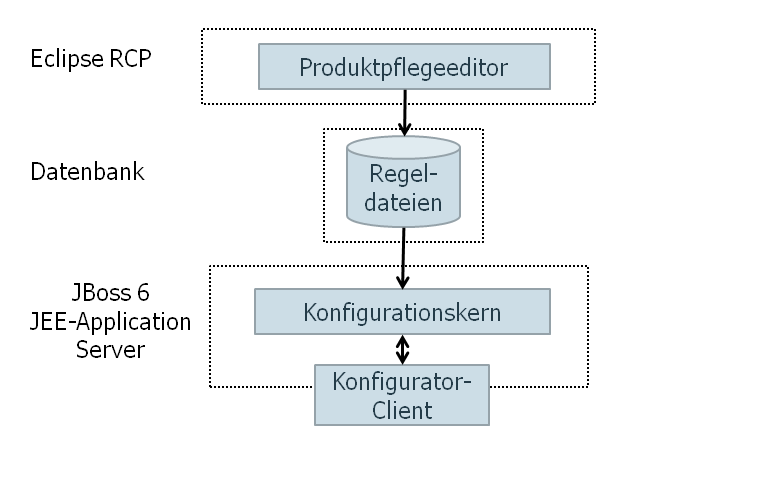
\includegraphics[width=\hsize]{images/AirbusAufbau}
\caption{Architektur der Airbus Komponenten}
\label{airbus_structure}
\end{figure}
Die Wissensverarbeitungs-Komponente aus Abschnitt \ref{konfiguratoren} ist hier der sogenannte \textit{Konfigurationskern}. Er ist für die Auswertung der getätigten Auswahl von Elementen des Produktes zuständig. Mithilfe von booleschen Regeln, welche mit dem \textit{Produktpflegeeditor} modelliert wurden und in einer \textit{Datenbank} gespeichert sind, wird die Auswahl verifiziert.
\par
 Der Konfigurationskern berechnet ebenfalls sogenannte Alternativen. Diese treten auf, sobald die derzeitige Selektion alleine, ohne Hinzunahme von weiteren Bauteilen, nicht umsetzbar ist. Der Konfigurator kann in diesem Fall neue Möglichkeiten (Alternativen) vorschlagen, damit die Konfiguration durchgeführt werden kann. Die Auswahl der Konfigurationselemente erfolgt im sogenannten Konfigurator-Client. Der Client ist mit der Benutzerschnittstelle im Expertensystem zu vergleichen. \par

Der Konfigurationskern, sowie der Client befinden sich auf einem Java-Applikations-Server. Der Produktpflegeeditor ist eine eigenständige Rich-Client Anwendung, welche auf dem Eclipse Rich-Client-Plattform Framework\cite{bib:eclipseRCP} basiert.

\subsection{Konfigurator des Kunden Airbus} \label{airbusConfigurator}
Die Arbeit wird speziell für den Flugzeughersteller Airbus\footnote{http://www.airbus.com/} angefertigt und beruht damit auf deren Konfigurationsmöglichkeiten. Airbus verwendet den Konfigurator für das Upgraden von bereits vorhandenen Flugzeugen einzelner Fluggesellschaften. Ein Beispiel für ein solches Upgrade können diverse Systemupgrades, wie bspw. ein neues Navigationssystem oder Ähnliches sein. Eine weitere Besonderheit im Konfigurationsprozess ist das Prüfen mit einzelnen Flugzeugen. Jedes verkaufte Flugzeug ist in der Datenbasis erfasst, sowie deren genaue Spezifikation und Bauteile. Der Konfigurator kann die Baubarkeit der einzelnen Upgrades genau auf ein bestimmtes Flugzeug prüfen lassen. \par

%TODO Beschreibung
 Bei der Modellierung von Konfigurationen werden sogenannte Status verwendet. Diese Status (engl. states) werden für Flugzeuge angelegt. Jeder einzelne Status repräsentiert eine erreichbare Konfiguration. Um einen Übergang zu einem state zu erreichen, wird ein bestimmtes Upgrade eingebaut  
 \par

Für die Konfiguration wird z.Zt. eine Weboberfläche als Konfigurations-Client verwendet. Diese Oberfläche ist sehr einfach gehalten und kann nur von Experten bedient werden, da mit einzelnen Produktcodes bei der Konfiguration gearbeitet wird. Die Weboberfläche befindet sich auf dem gleichen Applikationsserver wie der Kern und es besteht eine direkte Anbindung. In der Datenbank werden nicht nur Produkt- und Regelinformationen gehalten, sondern auch die Flugzeugdaten. 

  
\section{Mobile Anwendungen}

\subsection{Native Anwendungen}
\subsection{Web Anwendungen}
\subsection{Hybride Anwendung}


